%%%%%%%%%%%%%%%%%%%%%%%%%%%%%%%%%%%%%%%%%%%%%%%%%%%%%%%%%%%%%%%%%%%%%%%%%%%%%%%%%%%%%%%%%%%%%%%%%%%%%%%%%%%%%%%%%%%%%%%%%%%%%
\section{Introduction}\label{sec:introduction}


Wildfires are a growing problem in the United States and worldwide. The last decade has witnessed the costliest, the
most destructive and the deadliest wildland fires on record.



The remainder of my thesis is structured as follows:

\begin{itemize}
  \item In section \ref{sec:literature_review}.
  \item In section \ref{sec:detection} I propose a vision-based fire detection system. 
        I discuss the architecture and training of the underlying machine learning model in sections \ref{sec:model} and \ref{sec:training} respectively.
        I then perform both qualitative (\ref{sec:gradcam}) and quantitative (\ref{sec:eval}) evaluation of proposed model.


\end{itemize}


%%%%%%%%%%%%%%%%%%%%%%%%%%%%%%%%%%%%%%%%%%%%%%%%%%%%%%%%%%%%%%%%%%%%%%%%%%%%%%%%%%%%%%%%%%%%%%%%%%%%%%%%%%%%%%%%%%%%%%%%%%%%%
\section{Literature Review}\label{sec:literature_review}

  \subsection{The global wildfire emergency}

  Wildfires are a global problem. In the recent decades we observed some of the most severe wildland and record-braking fires on record. 
  
  Some of the most recent examples of unusually severe wildfires include:
  \begin{enumerate}
    \item 2019–20 bushfire season in Australia (spanning over 46M acres, over $6 \times$ the area of Belgium),
    \item 2019 Amazon Wildfires caused by excessive
    \item 2018 Camp Fire -- the deadliest and most destructive fire in California’s recorded history,
    \item 2020-21 wildfire season on the west coast of the United States.
          This event is already known to be the largest by area in California's recorded history.
  \end{enumerate}

  As depicted in figure \ref{fig:caltop20}, 17 out of the 20 largest wildland fires in California's recorded history happened over the last two decades (2000-2020).


  \begin{figure}\label{fig:caltop20}
    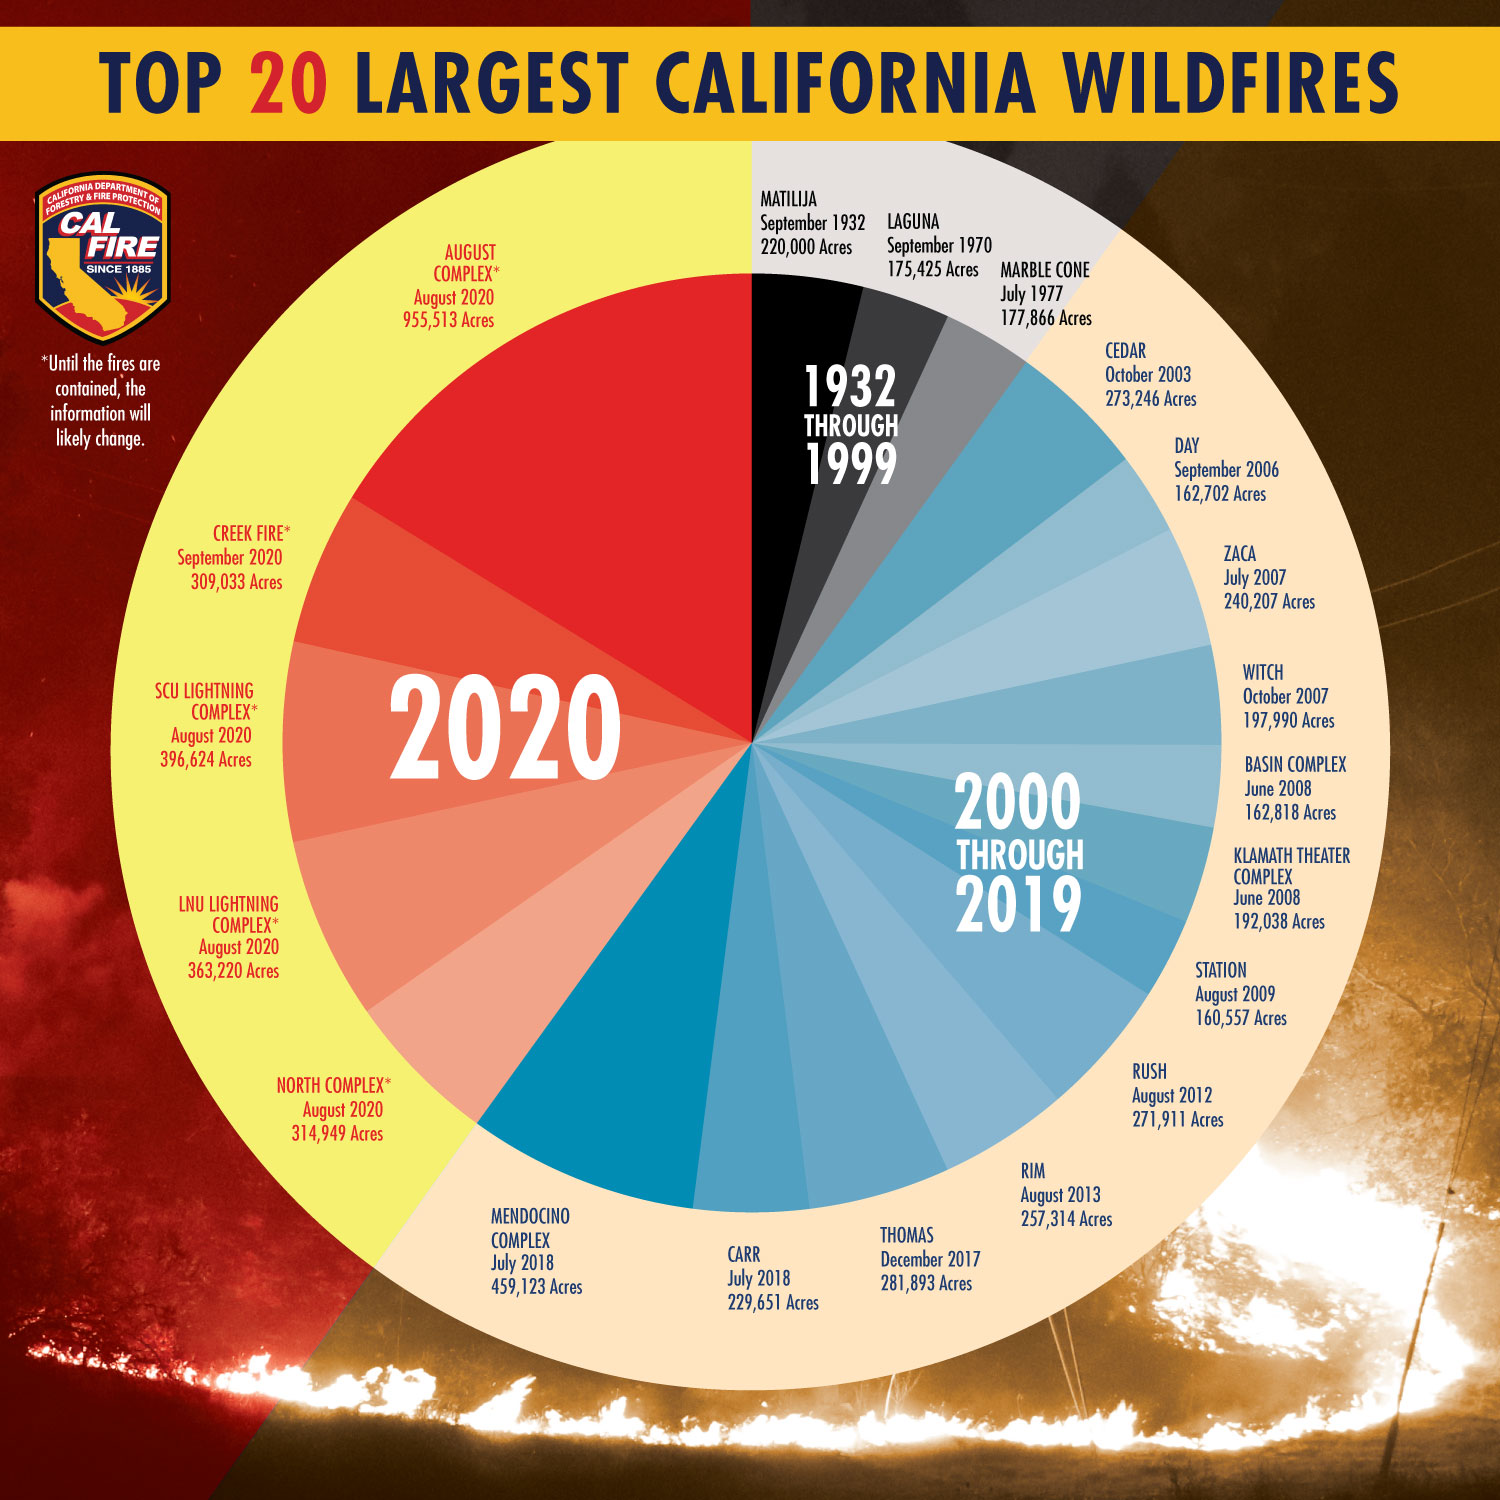
\includegraphics[width=0.5\linewidth]{calfire.jpeg}
    \caption{The 20 largest California wildfires on record, Image Credit: CAL FIRE\cite{calfire}}
  \end{figure}

  \begin{figure}
    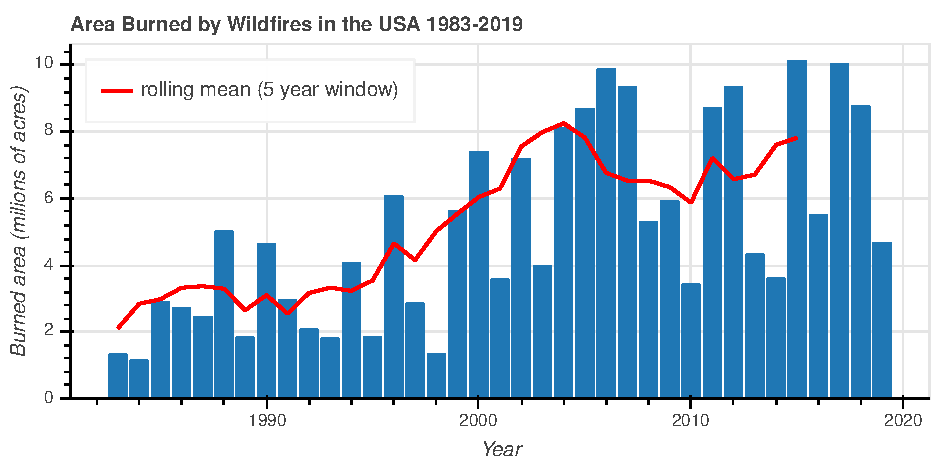
\includegraphics[width=\linewidth]{usa_burned_1983-2019.pdf}
    \caption{Area Burned by Wildfires in the USA (1983-2019), Data Source: National Interagency Coordination Center\cite{NICI}}
  \end{figure}

  \begin{figure}
    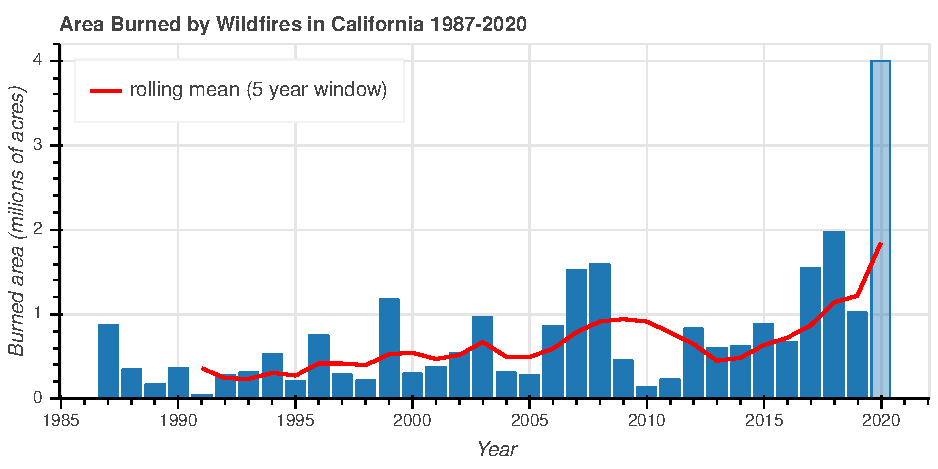
\includegraphics[width=\linewidth]{cali_burned_1987-2020.pdf}
    \caption{Area Burned by Wildfires in the USA (1983-2019). The data for 2020 as of Oct 1 2020, Data source: CAL FIRE\cite{calfire}}
  \end{figure}

  % https://www.epa.gov/outdoor-air-quality-data/air-data-daily-air-quality-tracker


  \subsection{Impact on humans and the Planet}

  Fires are an extremely dangerous phenomenon. 
  
  It is a human instinctve reaction to flee from uncontrolled fire.
  I personally have found it is truly awe-inspiring to stand in front blazing land fire.

  However, the implications for our health, climate might be 
  go far beyond the immediate danger posed by the flames.

  
  - human death (direct)
  - human death (indirect) %http://jhr.uwpress.org/content/44/4/916.short
  
  However, the direct deaths as a direct result of wildfires are perhaps only the tip of the iceberg.
  
  Wildland fires can contribute to human deaths in an indirect manner, via the severe air pollution.

  For example, Jayachandran~\cite{Jayachandran2009} has shown that the wildfire-caused severe air pollution during the 
  1997 Indonesian wildfire increased early-life (fetal, infant and child) mortality by 20 percent.
  In her study, Jayachandran found that the children of the poor parents were affected to a much greater extent than children of rich parents. %low-income




  - destruction of property
  - cost of wildfire supression

  - death of milions of animals, in some cases extinction of entire species\cite{}
  - shrinking of carbon sink
  - increased emissions of carbon dioxide and carbon monoxide %https://www.jpl.nasa.gov/spaceimages/details.php?id=PIA23356
  - periods of severe smoke/particulate matter related air pollution


  % Droughts, global warming, heatwaves Although global warming is not the 

  % For last few decades, we have been observing a growth in number of incidents, affected area, and suppression costs of wildland fires.
  
  % suggests that this issue might become even worse in the future.


  \subsection{Fire Detection with Computer Vision}

  \subsection{Existing Fire Image Datasets}

%%%%%%%%%%%%%%%%%%%%%%%%%%%%%%%%%%%%%%%%%%%%%%%%%%%%%%%%%%%%%%%%%%%%%%%%%%%%%%%%%%%%%%%%%%%%%%%%%%%%%%%%%%%%%%%%%%%%%%%%%%%%%
\section{Hardware Design}\label{sec:hardware}
  
  \subsection{Overview}
  Although not crucial

  \subsection{Drone}

  \subsubsection{Rationale for building custom UAV}

  The primary design consideration in building this system was enabling hardware-accelerated neural network inference on edge.
  There are few notable instances of using AI hardware accelerators in existing commercial drones.
  For example, DJI Mavic and DJI Phantom drones use Intel VPU chips for vision-based obstacle avoidance. 
  Another example is Skydio 2, which utilizes Nvidia Tegra TX2 processor for vision-based navigation and obstacle avoidance.

  Unfortunately, at the time of writing this thesis, there are no readily available low-cost drones that would provide developers and researchers
  programmatic access to the AI chip. 
  
  In the sections \ref{sec:sensors} I cover the design of the UAV platform, as well as the Camera-Compute Payload, enabling the system's perception.

  \subsubsection{Sensors}\label{sec:sensors}


  \paragraph{RTK GNSS}

  % TODO: image of stddev of two sensors

  \subsection{Payload}
  Talk about the payload 

%%%%%%%%%%%%%%%%%%%%%%%%%%%%%%%%%%%%%%%%%%%%%%%%%%%%%%%%%%%%%%%%%%%%%%%%%%%%%%%%%%%%%%%%%%%%%%%%%%%%%%%%%%%%%%%%%%%%%%%%%%%%%

\section{Fire Incident Aerial Image Dataset}\label{sec:dataset}

  \subsection{The rationale for creating a new datset}

  \subsection{Acquisiton}
  \begin{figure}
    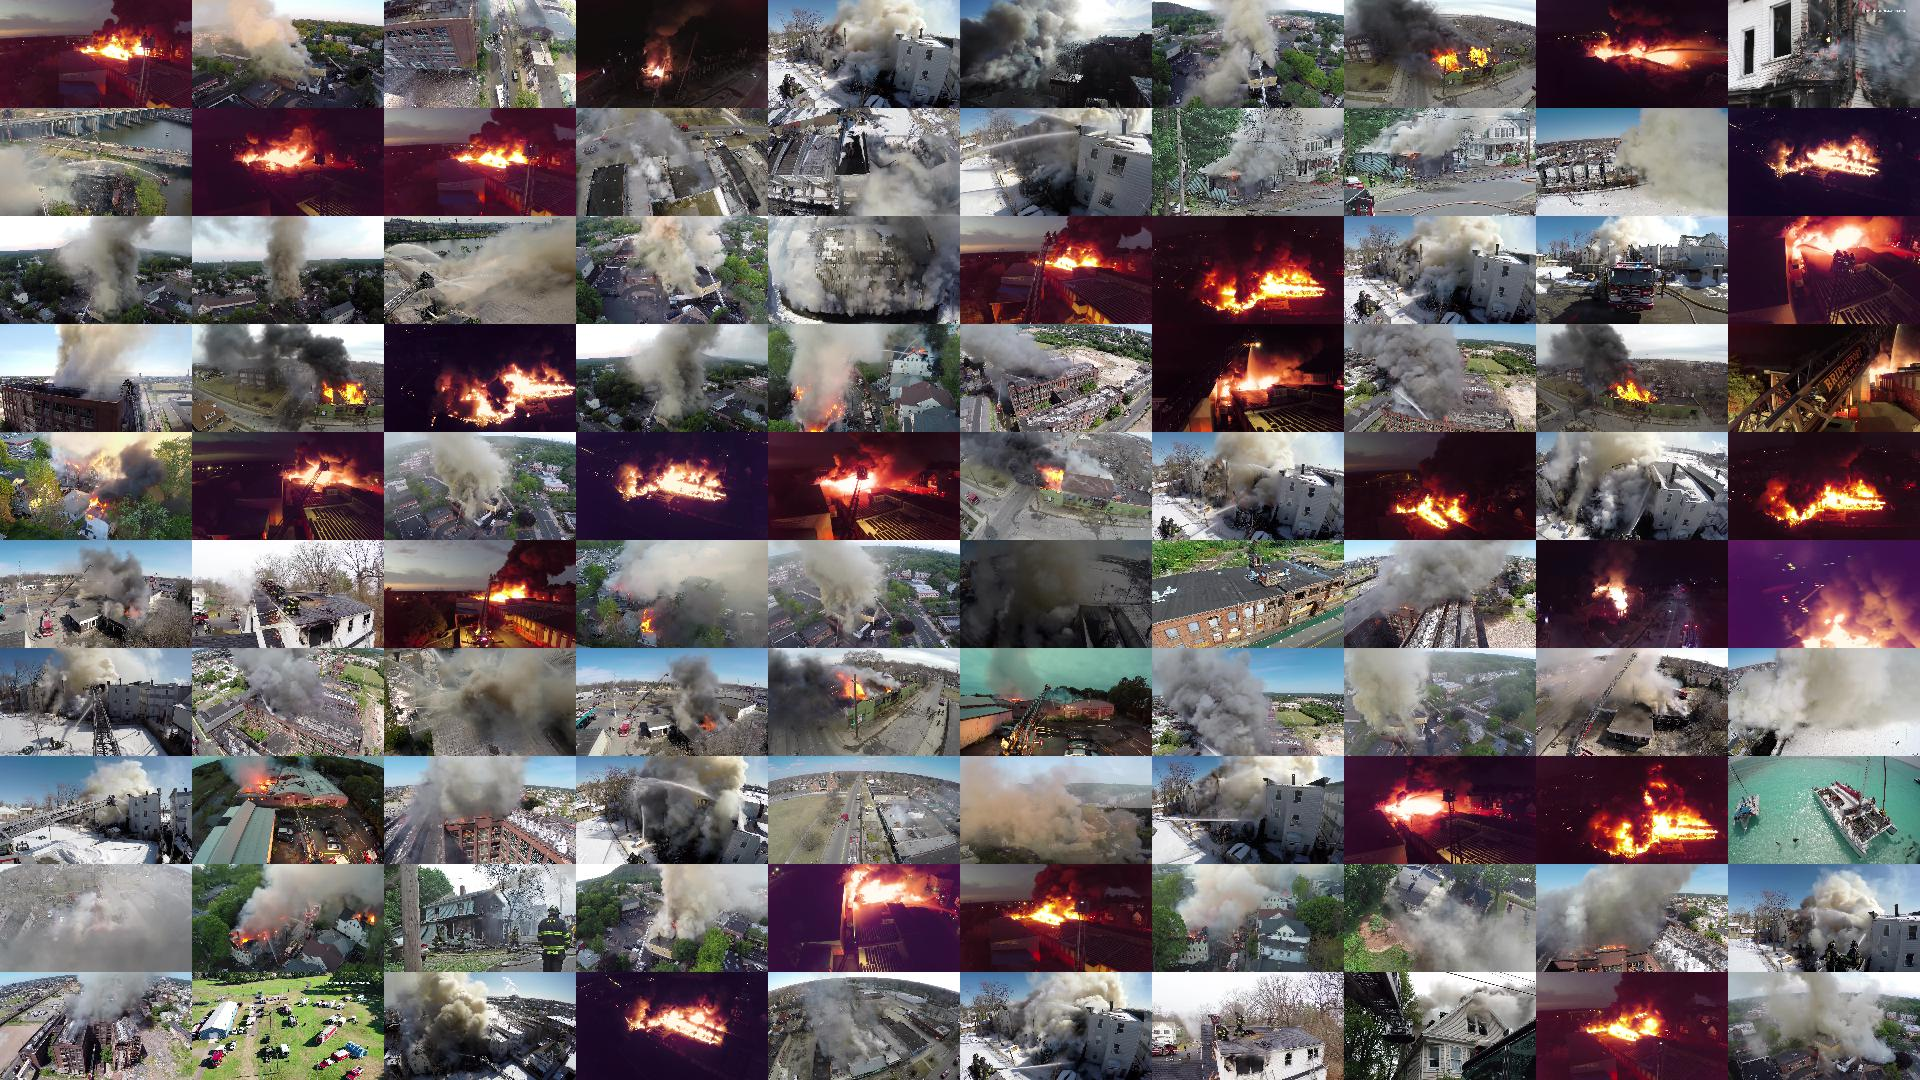
\includegraphics[width=\linewidth]{figures/lowres_100tiles.jpg}
    \caption{100 samples from the dataset}
  \end{figure}

  \subsection{Annotations}
  % TODO

\section{Fire Detection Model}\label{sec:detection}

  \subsection{Model}\label{sec:model}

  \subsection{Training}\label{sec:model}
    
  \subsection{Quantitative Evaluation}\label{sec:eval}

  \subsection{Qualitative Evaluation}\label{sec:gradcam}

\section{Auxilary Vision Systems}\label{sec:other}

  \subsection{Person Detection}

\section{Testing}

  \section{Field Testing}

  % Testing with Scott.
  The system was able to correctly classify $97\%$ of segments

  \section{End-to-end Simulation Testing}

%%%%%%%%%%%%%%%%%%%%%%%%%%%%%%%%%%%%%%%%%%%%%%%%%%%%%%%%%%%%%%%%%%%%%%%%%%%%%%%%%%%%%%%%%%%%%%%%%%%%%%%%%%%%%%%%%%%%%%%%%%%%%%
\section{Future Work}\label{sec:future_work}

  \subsection{RL control}

%%%%%%%%%%%%%%%%%%%%%%%%%%%%%%%%%%%%%%%%%%%%%%%%%%%%%%%%%%%%%%%%%%%%%%%%%%%%%%%%%%%%%%%%%%%%%%%%%%%%%%%%%%%%%%%%%%%%%%%%%%%%%%
\section{Conclusions}\label{sec:conclusions}


